El algoritmo de detección de tubos implementa una secuencia de cinco etapas que progresivamente extraen y refinan información estructural hasta identificar las líneas características.

\textbf{Etapa 1: Detección de bordes mediante Canny}

La primera etapa aplica el algoritmo de Canny, fundamentado teóricamente en la Sección 2.2.1 del marco teórico. El proceso inicia convirtiendo la imagen RGB a escala de grises y aplicando filtrado gaussiano con kernel de $5 \times 5$ píxeles para reducción de ruido. Sobre la imagen suavizada se calculan los gradientes de intensidad mediante operadores de Sobel.

La supresión de no-máximos adelgaza los bordes candidatos, preservando únicamente píxeles que son máximos locales en la dirección perpendicular al gradiente. Finalmente, la doble umbralización con histéresis clasifica píxeles en bordes fuertes y débiles. Los parámetros de umbralización se establecieron como $T_{bajo} = 20$ y $T_{alto} = 172$ tras experimentación empírica, valores que maximizan la detección de los bordes sutiles del tubo minimizando falsos positivos de ruido.

El resultado de esta etapa es una imagen binaria donde los píxeles blancos corresponden a transiciones abruptas de intensidad, típicamente concentrados en los bordes superior e inferior del tubo y en las interfaces con elementos de cultivo.

\textbf{Etapa 2: Filtrado por canal de saturación}

Los bordes detectados por Canny incluyen tanto los bordes objetivo (límites del tubo) como bordes espurios causados por vegetación, sombras de hojas y texturas del fondo. Para discriminar los bordes del tubo de otros elementos, se explota una propiedad cromática: el tubo de PVC blanco presenta saturación muy baja (color cercano al gris neutral), mientras que la vegetación presenta saturación moderada a alta debido a sus tonalidades verdes.

La imagen se transforma al espacio HSV y se extrae el canal S (saturación). Se invierte este canal mediante la operación $S_{inv} = 255 - S$, de modo que píxeles con baja saturación (tubo blanco) resulten en valores altos en el canal invertido. Se aplica umbralización con $T_S = 150$, generando una máscara binaria que aísla regiones de baja saturación.

Los bordes de Canny se filtran mediante operación AND binaria con esta máscara de saturación, preservando únicamente bordes que ocurren en regiones de baja saturación. Esta estrategia elimina efectivamente los bordes causados por vegetación verde, que presenta alta saturación.

\textbf{Etapa 3: Refinamiento morfológico}

Los bordes filtrados presentan típicamente discontinuidades causadas por variaciones locales de iluminación o por oclusiones parciales debidas a hojas que cubren pequeñas secciones del tubo. Para conectar segmentos de borde fragmentados se aplica operación de cierre morfológico con elemento estructurante rectangular de $3 \times 9$ píxeles.

La orientación vertical del kernel (mayor altura que ancho) favorece la conexión de segmentos de líneas horizontales mientras preserva la separación entre líneas vertical. Esta operación es crítica para que la subsecuente detección de contornos identifique el tubo como una región conexa única en lugar de múltiples fragmentos independientes.

\begin{figure}[H]
\centering
\begin{subfigure}[b]{0.48\textwidth}
    \centering
    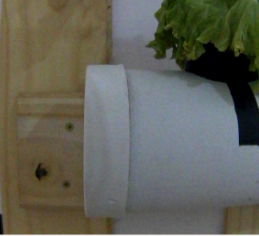
\includegraphics[width=\textwidth]{imagenes/detector_tubos_1_original.png}
    \caption{Imagen RGB original}
\end{subfigure}
\hfill
\begin{subfigure}[b]{0.48\textwidth}
    \centering
    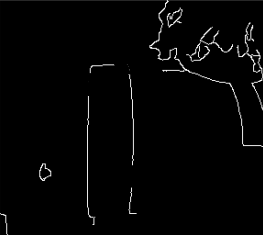
\includegraphics[width=\textwidth]{imagenes/detector_tubos_2_canny.png}
    \caption{Bordes Canny (T=20-172)}
\end{subfigure}

\vspace{0.3cm}

\begin{subfigure}[b]{0.48\textwidth}
    \centering
    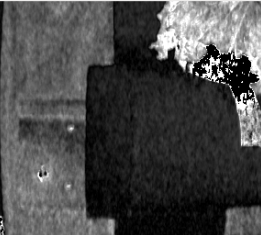
\includegraphics[width=\textwidth]{imagenes/detector_tubos_3_canal_s.png}
    \caption{Máscara de baja saturación}
\end{subfigure}
\hfill
\begin{subfigure}[b]{0.48\textwidth}
    \centering
    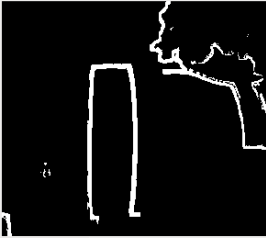
\includegraphics[width=\textwidth]{imagenes/detector_tubos_5_morfologia.png}
    \caption{Morfología de cierre (kernel 3×9)}
\end{subfigure}

\vspace{0.3cm}

\caption{\textit{Procesamiento del detector de tubos mostrando las transformaciones sucesivas hasta la identificación de bordes del tubo}}
\label{fig:proceso_tubos}
\end{figure}

\textbf{Etapa 4: Detección de contornos y scoring}

Sobre la imagen de bordes refinados se ejecuta el algoritmo de detección de contornos de Suzuki-Abe. Los contornos detectados se filtran aplicando criterio de área mínima de 250 píxeles, eliminando pequeñas regiones de ruido residual.

Para cada contorno que supera el filtrado de área se calcula su rectángulo delimitador y se evalúa la relación de aspecto $AR = w/h$. Los tubos, al observarse desde una perspectiva frontal, presentan geometría predominantemente vertical, resultando en relaciones de aspecto $AR < 0.9$. Contornos con $AR \geq 0.9$ se descartan por corresponder a elementos horizontales o cuadrados.

Los contornos candidatos (verticales) se someten a un sistema de scoring que evalúa simultáneamente tres criterios. El primer criterio considera la relación de aspecto: valores $AR < 0.5$ (fuertemente verticales) reciben 35 puntos, valores $0.5 \leq AR < 0.7$ reciben 25 puntos, y valores $0.7 \leq AR < 0.9$ reciben 15 puntos. El segundo criterio evalúa el área normalizada del contorno, favoreciendo áreas intermedias consistentes con el tamaño esperado del tubo. El tercer criterio analiza la homogeneidad de la saturación dentro de la región delimitada: regiones con baja desviación estándar de saturación (color uniforme) reciben puntuación mayor.

El contorno con mayor puntuación total se selecciona como el tubo objetivo.

\begin{figure}[H]
    \centering
    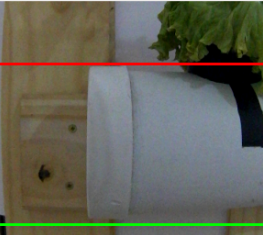
\includegraphics[width=0.48\textwidth]{imagenes/detector_tubos_6_lineas.png}
    \caption{\textit{Líneas superior e inferior detectadas}}
    \label{fig:detector_tubos_lineas}
\end{figure}

\subsubsection{Consideraciones de robustez}

El algoritmo implementa mecanismos de validación para garantizar robustez ante casos ambiguos. Cuando no se detectan contornos válidos (ningún contorno cumple los criterios de área, relación de aspecto y scoring), el sistema retorna valores nulos indicando ausencia de tubo en el campo de visión. Esto ocurre naturalmente cuando el robot se posiciona entre tubos o cuando las condiciones de iluminación son extremadamente deficientes.

Cuando se detectan múltiples contornos candidatos con puntuaciones similares (diferencia menor al 10 por ciento), el sistema genera una advertencia de detección ambigua pero procede seleccionando el contorno de mayor score. Esta situación puede ocurrir cuando hay elementos estructurales del invernadero (postes, soportes) que presentan geometría y propiedades cromáticas similares a los tubos.

El tiempo total de procesamiento del pipeline completo es de aproximadamente 120 milisegundos, desglosado en: conversión a escala de grises y filtrado gaussiano (12 ms), detección de bordes Canny (35 ms), conversión a HSV y extracción de canal S (15 ms), umbralización y operación AND (8 ms), morfología de cierre (18 ms), detección de contornos (20 ms), y cálculo de scoring y extracción de coordenadas (12 ms).
